\chapter{ORM}

Per la parte relativa al database si è scelto di utilizzare la tecnica ORM (Object-Relational Mapping) per facilitare l'integrazione di database relazionali con software aderenti al paradigma della programmazione orientata agli oggetti. L'ORM si pone infatti come layer intermedio fra un servizio (in questo caso l'applicazione) e il database utilizzato dal servizio (in questo caso MySQL). Di seguito verranno analizzati i vantaggi e gli svantaggi di tale tecnica, in che contesti è conveniente utilizzarla e perché si è scelto di implementarla nell'applicazione oggetto di questa tesi; infine saranno mostrati degli stress tests volti a confrontare le performance di ORM e JDBC.

\section{Vantaggi}

Usare la tecnica ORM risulta vantaggiosa in termini di:

\begin{itemize}
  \item produttività
  \item progettazione del codice
  \item testing
  \item versatilità
  \item gestione della cache 
  \item sicurezza
  \item ecosistema
  \item gestione delle query
\end{itemize}

Di seguito si analizza ognuno dei punti precedenti più nel dettaglio.

Produttività: senza l'ORM, l'ingegnere del software che progetta l'applicazione deve occuparsi anche della scrittura del corrispondente codice SQL; in particolare, a seconda del database utilizzato, il linguaggio SQL specifico può essere diverso e deve essere conosciuto dal programmatore. La scrittura di statements SQL può richiedere molto tempo, delegandola all'ORM si permette all'ingegnere del software di occuparsi solo della parte di codice relativa al linguaggio a oggetti, riducendo il tempo necessario allo sviluppo dell'intera applicazione e, di conseguenza, il suo time-to-market. L'ORM è quindi particolarmente indicato per i progetti che hanno vincoli di tempo cruciali per il successo del prodotto, come per esempio nel caso di prodotti che devono essere lanciati per la prima volta sul mercato. Permette inoltre di gestire automaticamente operazioni comuni come CRUD (Create, Read, Update, Delete), con conseguente risparmio di tempo e impegno. 

Progettazione del codice: nel momento in cui si implementa correttamente l'ORM, esso induce anche l'utilizzo di design patterns che fanno uso di best practices per la progettazione dell'applicazione. Si ottiene quindi un codice meglio strutturato e più facilmente comprensibile, ciò semplifica anche la sua manutenzione, che è l'aspetto chiave per il successo (anche in termini economici) del software e il suo aggiornamento.

Testing: dal momento che l'ORM si occupa di generare il codice SQL necessario, una volta che è stato testato il codice per l'accesso ai dati, non è necessario testarlo nuovamente a meno che non venga cambiata la logica con cui i dati sono acceduti. Molti ORM permettono inoltre di gestire i test in maniera tale da garantire che non lascino dati residui nel database.

Versatilità: la generazione del codice ad opera dell'ORM permette di cambiare facilmente database senza la necessità di modificare il codice; nel caso specifico dell'applicazione in esame, è possibile passare facilmente da MySQL (utilizzato per la versione desktop) a SQLite per una versione mobile. Sarà infatti l'ORM che si occuperà della generazione del codice nell'SQL proprio del nuovo database selezionato.

Gestione della cache: essendo le entità salvate in memoria è necessario meno tempo per il loro caricamento sul database e si riduce il numero di query effettuate.

In generale, come linea guida si può affermare che l'utilizzo di ORM sia particolarmente indicato nel caso in cui gli oggetti e le modalità di accesso ad essi non siano particolarmente complessi. Per query semplici, come per esempio la restituzione di oggetti dal database, l'impiego di ORM permette di risparmiare molto tempo. Sebbene vi siano diversi ORM (fra cui Hibernate) che permettono di accedere alla connessione al database molto facilmente, se vi è necessità di numeroso codice SQL specifico dell'applicazione il rischio è quello di non sfruttare appieno l'ORM (il cui obiettivo è proprio minimizzare la scrittura di codice SQL).

Sicurezza: se non c'è una appropriata validazione dei valori in input (come possono essere, ad esempio, quelli dei cookies) prima di passarli a delle query SQL eseguite dal database, ci si espone al rischio di un attacco tramite SQL injection, una delle più semplici e potenzialmente una delle più pericolose minacce per la sicurezza di un'applicazione. Questa eventualità può essere scongiurata tramite l'utilizzo di un ORM (a patto che non vi sia del puro SQL in altre parti dell'applicazione) dal momento che spesso fa uso di query parametrizzate, tuttavia non è strettamente necessario ed uno sviluppatore esperto può facilmente risolvere questo problema senza il bisogno di ricorrere a un ORM.

Ecosistema: ORM popolari hanno spesso ampie communities, offrono plugins, estensioni e supporto che possono accelerare lo sviluppo dell'applicazione.

Gestione delle query: molti ORM offrono costruttori di query o linguaggi specifici per un particolare dominio, che semplificano la creazione di query complesse rendendole più leggibili e mantenibili.

\section{Svantaggi}

Fra gli svantaggi da considerare se si utilizza l'ORM vi sono:

\begin{itemize}
\item performance overhead
\item controllo limitato
\item curva di apprendimento
\item problematiche di astrazione
\item problemi di scalabilità
\item problemi di compatibilità
\item complessità del mapping
\item problemi di sicurezza
\end{itemize}

Di seguito si analizza ognuno dei punti precedenti più nel dettaglio.

Performance overhead: l'ORM genera spesso query SQL complesse che possono essere meno efficienti rispetto a query SQL scritte direttamente, questo si nota soprattutto con datasets molto grandi o operazioni complesse.

Controllo limitato: adattare le query SQL in funzione delle performance è più difficile con l'ORM, dal momento che esso astrae l'SQL sottostante. Inoltre l'ORM fornisce un approccio comune a tutti i database, limitando l'uso di funzionalità avanzate specifiche di un certo DBMS ed eventuali ottimizzazioni.

Curva di apprendimento: imparare come un ORM mappa l'SQL può essere complesso, comprendere le implicazioni sulle performance e le best practices richiede molto tempo. Identificare problemi durante il debugging può essere più difficile poiché gli sviluppatori devono avere cognizione sia delle astrazioni dell'ORM che delle query SQL sottostanti che esso genera.

Problematiche di astrazione: le differenze concettuali tra la programmazione orientata agli oggetti e i database relazionali può portare a modelli inefficienti, inoltre il comportamento dell'ORM potrebbe differire da quello atteso, specialmente quando si trova a gestire query personalizzate o relazioni complesse fra le entità.

Problemi di scalabilità: l'ORM può incontrare difficoltà legate alla scalabilità con datasets molto grandi o applicazioni fortemente concorrenti, dove l'ottimizzazione di query e database è cruciale.

Problemi di compatibilità: mantenere la libreria ORM aggiornata con la versione del database può essere difficile, gli aggiornamenti possono causare l'insorgere di incompatibilità. Inoltre i cambiamenti nella stessa libreria ORM possono introdurre modifiche che richiedono un refactoring significativo del codice.

Complessità del mapping: gestire concetti complessi legati alla programmazione orientata agli oggetti come ereditarietà e polimorfismo può essere inefficiente in un contesto come quello dei database relazionali che non li prevedono, inoltre modificare lo schema del database in parallelo con gli oggetti che vengono memorizzati può essere complesso e condurre facilmente ad errori; è pertanto necessario pianificare delle accorte strategie di migrazione.

Problemi di sicurezza: una configurazione errata o un utilizzo improprio dell'ORM può comunque introdurre vulnerabilità, inoltre le query generate automaticamente potrebbero non essere state accuratamente testate per determinate funzioni di sicurezza rispetto a query SQL scritte a mano.

\newpage

\section{Stress tests e conclusioni}

Di seguito vengono proposti (prima in forma tabellare e poi in forma grafica) una serie di test volti a verificare la differenza di prestazioni fra l'applicazione che non fa uso di ORM e la versione dell'applicazione che lo utilizza. In particolare, si considera come task l'inserimento di prodotti nel database. 

\begin{table}[h!]
  \begin{center}
    \caption{Stress tests in forma tabellare.}
    \begin{tabular}{l|c|r} % <-- Alignments: 1st column left, 2nd middle and 3rd right, with vertical lines in between
      \textbf{Numero di prodotti} & \textbf{Tempo (Non-ORM)} & \textbf{Tempo (ORM)}\\
      \hline
      1K & $\sim$ 0.6 secondi & $\sim$ 1.5 secondi\\
      10K & $\sim$ 2 secondi & $\sim$ 4 secondi\\
      100K & $\sim$ 14 secondi & $\sim$ 25 secondi\\
      1M & $\sim$ 134 secondi & $\sim$ 231 secondi\\
    \end{tabular}
  \end{center}
\end{table}

\begin{figure}[H]
  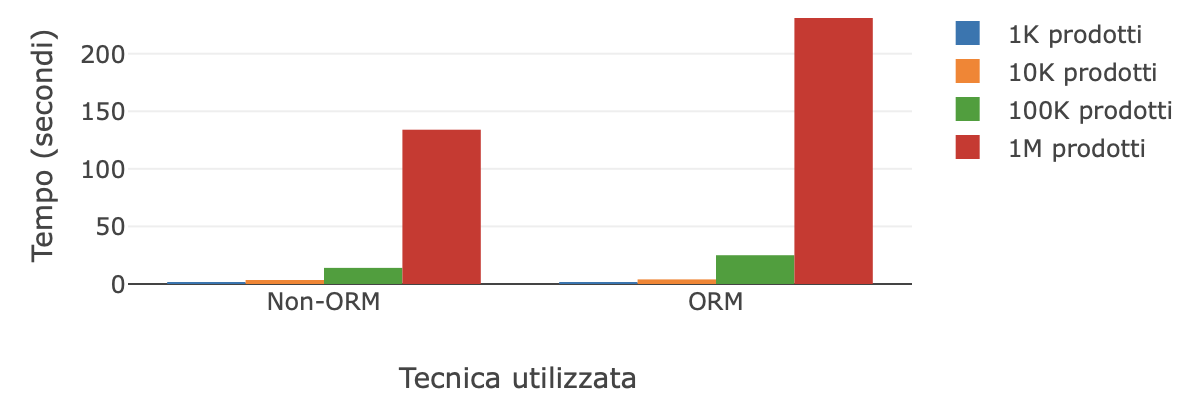
\includegraphics[width=\linewidth]{images/stress-tests-diagram.png}
  \caption{Stress tests in forma grafica.}
  \label{fig:stresstests}
\end{figure}

Appare evidente come l'overhead in caso di grandi quantità di dati appaia non trascurabile e risulti nell'impossibilità pratica di utilizzare l'ORM. Tuttavia, nel caso di quantità di dati relativamente ridotte, seppur presente esso è impercettebile per l'utente. Nel caso in esame, essendo gli oggetti inseriti nel database i prodotti presenti nella dispensa di un utente, ed essendo le operazioni svolte su di essi molto semplici, è improbabile che si raggiungano numeri tali da far sperimentare all'utilizzatore dell'applicazione un evidente calo di prestazioni, mentre per il programmatore l'utilizzo di ORM semplifica notevolmente lo sviluppo, la manutenzione e il testing del codice.
